\documentclass[Aflevering]{subfiles}
\begin{document}


\chapter{Problemstilling}


Med dette projekt �nskes at opn� et system, hvor en bruger med et tastatur kan genere toner fra tastetryk.
Tastaturet vil v�re forbundet til DE2-boardet, som behandler inputtet fra tastaturet og generer tonerne p� baggrund af disse.
\\
\\
Systemet opbygges s�ledes, at et tastatur med PS/2-udgang forbindes til DE2-boardet, hvorp� der sidder en FPGA af typen \textit{Cyclone II}.
Tilsluttet til DE2-boardet er ogs� et par h�jtalere forbundet via mini-jack stik.
\\
\\
Intentionen med opstillingen er, at der ved et tastetryk p� tasteturet bliver genereret en tone, en sinuskurve, som adskiller sig for hver knap.
\\
\\
Der oprettes en microprocessor, som bl.a. har forbindelse til driveren for tasteturet. 
Driveren til tasteturet er tredjeparts software.
\\
Gennem microprocessoren sendes tastetryk vha. \textit{C}-kode til \textit{VHDL}-koden, der indeholder en sinusgenerator.
Derudover kan der ogs� sendes kommandoer fra en konsol til sinusgeneratoren.
\\
Fra sinusgeneratoren sendes lyden ud til h�jtalerne via \textit{ST-bussen}, bit for bit.
\\
\\
Frekvensen der afspilles vises p� 7-segments displayet og p� det store display vises en fyldig tekst vedr. frekvensen.
\\
\\
Herunder ses opstillingen:
\begin{figure}[hbtp]
\centering
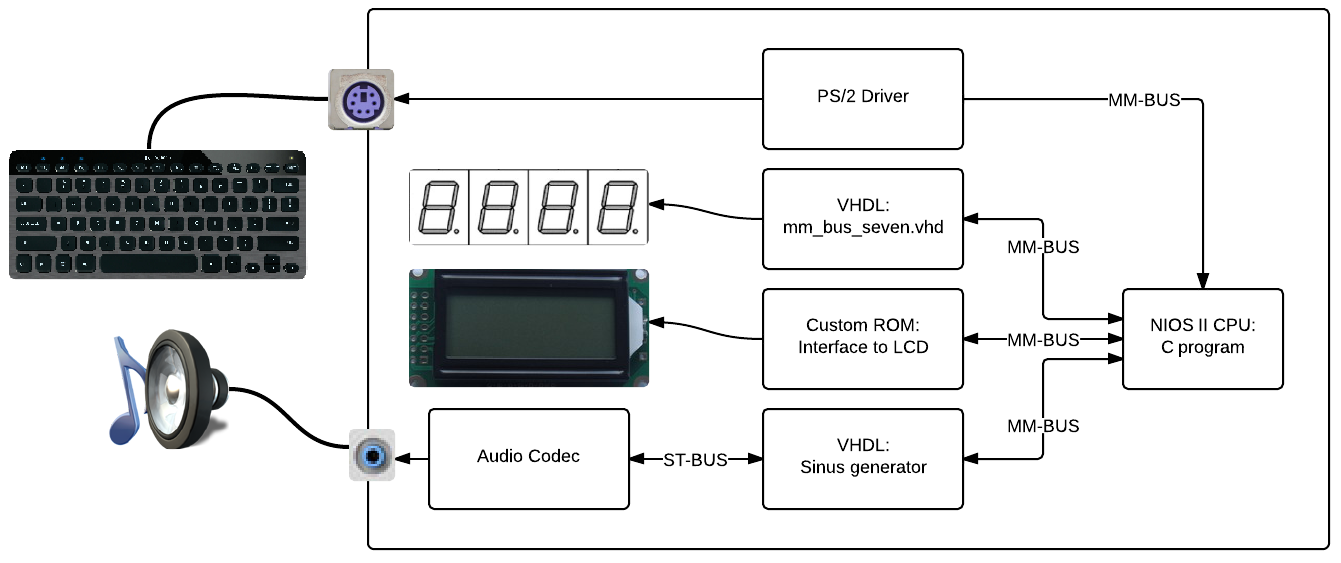
\includegraphics[scale=0.4]{Opstilling.png}
\caption{Opstilling}
\end{figure}


%\section{Brugbare ting}
%C:\altera\12.1\ip\University_Program\Input_Output\
%altera_up_avalon_ps2\doc

%C:\altera\12.1\University_Program\
%NiosII_Computer_Systems\DE2\DE2_Media_Computer\doc




\end{document} 